\documentclass[english]{beamer}
\usepackage[utf8]{inputenc}
\usepackage[english]{babel}
\usepackage{multicol}
\usepackage{tikz}
\usepackage{multirow}
\usepackage{changepage}
\usepackage{subcaption}
\captionsetup{compatibility=false}

\usepackage{caption}
\captionsetup[figure]{labelformat=empty}

\usetheme[language=english,footline=sections,faculty=tw,usecolors,framenumber,totalframenumber]{UniversiteitGent}

\setbeamertemplate{caption}{\raggedright\insertcaption\par}
\setbeamertemplate{footline}
{
	\leavevmode%
	\hbox{%
		\begin{beamercolorbox}[wd=.333333\paperwidth,ht=2.25ex,dp=1ex,center]{author in head/foot}%
			\usebeamerfont{author in head/foot}\insertsection
		\end{beamercolorbox}%
		\begin{beamercolorbox}[wd=.333333\paperwidth,ht=2.25ex,dp=1ex,center]{title in head/foot}%
			\usebeamerfont{title in head/foot}\insertsubsection
		\end{beamercolorbox}%
		\begin{beamercolorbox}[wd=.333333\paperwidth,ht=2.25ex,dp=1ex,right]{date in head/foot}%
%			\usebeamerfont{date in head/foot}\insertshortdate{}\hspace*{2em}
			\insertframenumber{} / \inserttotalframenumber\hspace*{2ex} 
		\end{beamercolorbox}}%
		\vskip0pt%
	}

\usetikzlibrary{arrows}
\usetikzlibrary{fit}
\usetikzlibrary{calc}
\usetikzlibrary{backgrounds}
\usetikzlibrary{shapes.geometric}
\usetikzlibrary{positioning}

\tikzset{hide on/.code={\only<#1>{\color{white}}}}
\tikzset{
	invisible/.style={opacity=0},
	visible on/.style={alt=#1{}{invisible}},
	alt/.code args={<#1>#2#3}{%
		\alt<#1>{\pgfkeysalso{#2}}{\pgfkeysalso{#3}} % \pgfkeysalso doesn't change the path
	},
	level/.style={sibling distance = 4cm/#1,level distance = 1.5cm},
	treenode/.style = {align=center, inner sep=0pt, text centered,
		font=\ttfamily},
	arn_l/.style = {treenode, circle, ugentblue, draw=ugentblue, fill=ugentyellow,
		text width=1.5em, very thick},% leaf node
	arn_x/.style = {treenode, circle, white, draw=ugentblue, fill=ugent-pp,
		text width=1.5em, very thick},% red
	arn_y/.style = {treenode, circle, white, draw=ugentblue, fill=ugent-tw,
		text width=1.5em, very thick},% blue
	arn_0/.style = {treenode, draw=none,
		fill=none, text width=0},% hidden node
	arn_s/.style = {treenode, circle,
		fill=ugentblue, text width=0.75em},%small node
	rect_l/.style ={shape=rectangle, rounded corners, draw, align=center,
		color=ugentblue, top color=ugentyellow, bottom color=ugentyellow, very thick},
	rect_x/.style ={shape=rectangle, rounded corners, draw, align=center,
		color=ugentblue, top color=ugent-pp, bottom color=ugent-pp, very thick},
}


\AtBeginSection[]
{
	\begin{frame}
		\begin{columns}[t]
			\begin{column}{5cm}
				\tableofcontents[sections={1-4},currentsection, hideothersubsections]
			\end{column}
			\begin{column}{5cm}
				\tableofcontents[sections={5-8},currentsection,hideothersubsections]
			\end{column}
		\end{columns}
	\end{frame}
}


\title{Design of a diagnosis and follow-up platform for patients with chronic headaches}
%\subtitle{Phylogeny Comparison}
\author{Kiani Lannoye \& Gilles Vandewiele}
\mode<beamer>{\institute{Faculty of Engineering and Architecture}}

\begin{document}
\begin{frame}
	\titlepage
\end{frame}

%\begin{frame}
%	\begin{columns}[t]
%		\begin{column}{5cm}
%			\tableofcontents[sections={1-4},currentsection, hideothersubsections]
%		\end{column}
%		\begin{column}{5cm}
%			\tableofcontents[sections={5-8},currentsection,hideothersubsections]
%		\end{column}
%	\end{columns}
%\end{frame}

\section{Intro}
\label{sec:intro}
\begin{frame}{Headaches}
	\begin{figure}[!h]
		\begin{tikzpicture}[sibling distance=10em,
		every node/.style = {shape=rectangle, rounded corners,
			draw, align=center,
			top color=white, bottom color=blue!20}]]

		\node<1>{
			\centering
			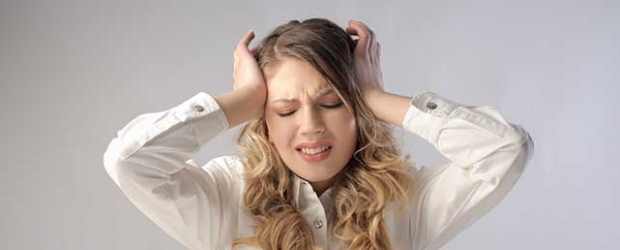
\includegraphics[width=\textwidth]{figures/headache.jpg}
			};
		\node<2-> {Headaches}
		child[visible on=<3->] { 
			node {Primary headaches} 
				child[visible on=<5->] {
					node {Migraine}
						child[visible on=<6->] {
							node {Aura}
						}
						child[visible on=<6->]{
							node {No aura}
						}
				}
				child[visible on=<5->] {
					node {Tension}
				}
				child[visible on=<5->] {
					node {Cluster}
				}
		}
		child[visible on=<4->] { node {Secondary headaches}};
		\end{tikzpicture}
	\end{figure}
\end{frame}
\subsection{Current process UH Ghent}

\begin{frame}{Current process UH Ghent}
	Current process at UH Ghent is:
	\begin{itemize}
		\item Not digital
		\item cumbersome
		\item long-lasting
	\end{itemize}
\end{frame}

\begin{frame}
	\framesubtitle{Current process at UH Ghent}
	\begin{figure}[!h]
		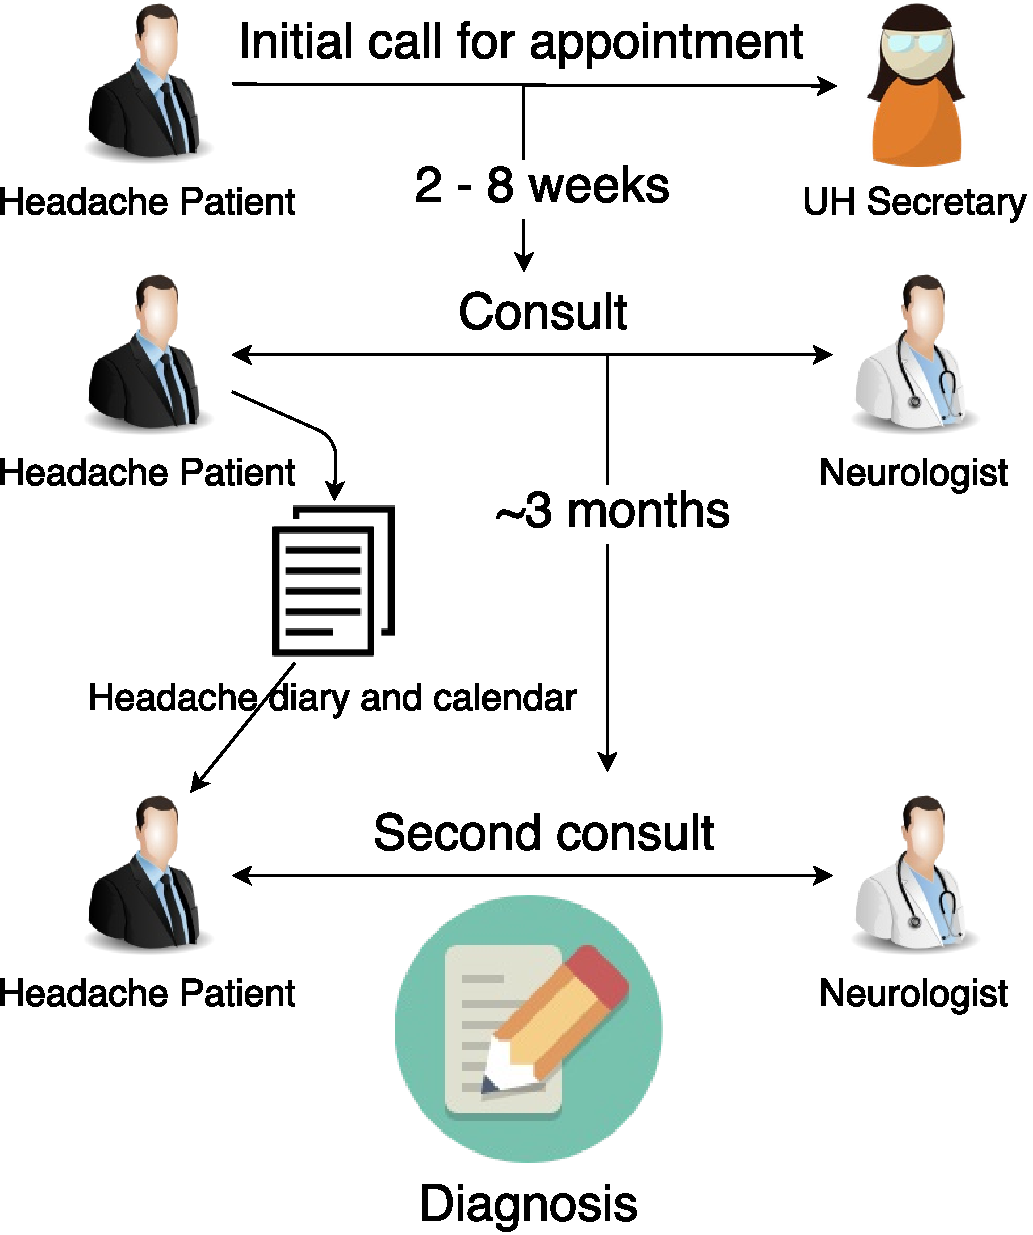
\includegraphics[width=0.5\textwidth]{figures/UZ_patient.pdf}
	\end{figure}
\end{frame}

\begin{frame}
	So there is need for a better (digital) alternative! This alternative has to:
	\begin{itemize}
		\item capture at least the same information as current solution
		\item be more efficient
		\item provide a second opinion for the doctors (auto-diagnose)
	\end{itemize}
\end{frame}
% section intro (end)
\section{Platform requirements}
\label{sec:platform_req}
\begin{frame}
	\frametitle{Platform requirements}


		Our proposed alternative consists of:
		\begin{itemize}
			\item Headache journal: mobile app
			\item Doctor Dashboard: web application
			\item Machine learning module: decision support
		\end{itemize}
		\ \newline
		Solution non-functional requirements:
		\begin{itemize}
			\item Security
			\item Availability
			\item Performance \& learning curve
			\item Usability
		\end{itemize}
\end{frame}
\begin{frame}
		\frametitle{Platform requirements}
		\begin{figure}[!h]
			\includegraphics[width=\textwidth]{figures/system_analysis.png}
		\end{figure}	
	
\end{frame}
% section Platform requirements (end)
\section{Mobile application}
\begin{frame}{Mobile Application}
	\centering
	\begin{figure}
		\only<1>{		\includegraphics[width=\textwidth]{figures/system_analysis.png}}
		\only<2>{
			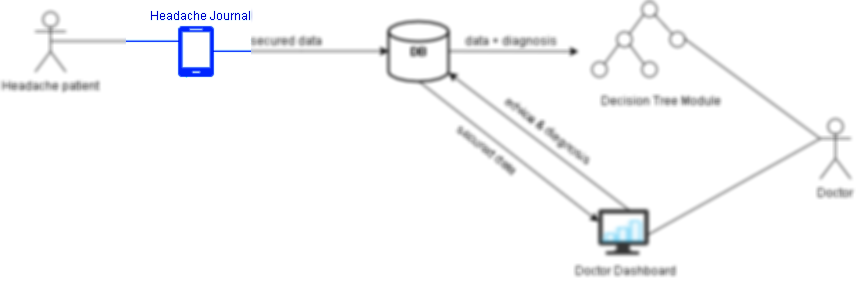
\includegraphics[width=\textwidth]{figures/system_analysis_mobile_app.png}
		}
	\end{figure}
\end{frame}
\begin{frame}{Mobile Application}
	Why create a new application? 
	\begin{block}{Competition}{}
		\begin{itemize}
			\item Migraine Buddy
			\item Headache Diary
			\item Pfizer headache journal
		\end{itemize}
	\end{block}
	\pause
	All good, but:
	\pause
	\begin{itemize}
		\item none captures all data needed
		\item none offers usable data export
	\end{itemize} 
\end{frame}
%\subsection{Development paradigms}
%\begin{frame}{Development paradigms}
%	Different kinds of approaches for mobile application development:
%	\begin{itemize}
%		\item Web application
%		\item Hybrid application
%		\item Native application
%	\end{itemize}
%	$\rightarrow$ How do we choose?
%\end{frame}
%\begin{frame}{Web application}
%	Webapps are developed once and can be viewed on (almost) all smartphones (via built-in web engine).\newline
%	\newline
%	$+$ ``write once, run everywhere'' $\Rightarrow$ lower cost\newline
%	$+$ No installation required\newline
%	$-$ limited use of device specific features (GPS, camera, ...)\newline
%	\textbf{$-$ Not all devices same web engines $\Rightarrow$ other view}\newline
%	$-$ No native look and feel\newline
%	\newline
%	{\Large \color{red}  $\Rightarrow$ No web application}
%\end{frame}
%
%\begin{frame}{Native application}
%	Native apps are developed once for each OS and installed on the device.\newline
%	\newline
%	$+$ Best performance (optimized machine code at compile time)\newline
%	$+$ Device specific features usable (GPS, camera, ...)\newline
%	$+$ Native look and feel\newline
%	\textbf{$-$ Write code for each OS (very costly dev + maintenance)}\newline
%	$-$ Installation required\newline
%	\newline
%	{\Large \color{red}  $\Rightarrow$ Native application?}
%\end{frame}
%
%\begin{frame}{Hybrid application}
%	Hybrid apps are developed once and installed on the device. It uses the devices internal web engine, but has more control than web applications.\newline
%	\newline
%	$+$ ``write once, run everywhere'' $\Rightarrow$ lower cost\newline
%	$+$ Better performance (semi-optimized machine code)\newline
%	$+$ Device specific features usable (GPS, camera, ...)\newline
%	$+$ Native look and feel (using libraries)\newline
%	$-$ Installation required\newline
%	\textbf{$-$ Not all devices same web engines $\Rightarrow$ other view\newline (but manageable)}
%		\vspace{0.8em}
%
%	{\Large \color{red}  $\Rightarrow$ Hybrid application?}
%\end{frame}

\begin{frame}{Cross platform vs Native}
	\only<2>{}
\begin{tabular}{l||ll}
	& \textbf{\color<2>{red}Native}                                                                                                                          & \textbf{\color<2>{green}Cross-platform}                                                                                                                                                                            \\ \hline \hline
	\textbf{+}    & \begin{tabular}[c]{@{}l@{}}+ Native UX\\ + device-specific features\\ + Better performance\end{tabular}               & \begin{tabular}[c]{@{}l@{}}+ 1 language\\ + Write once, run everywhere\\ + Less maintenance\end{tabular}                                                                \\ \hline
	\textbf{-} & \begin{tabular}[c]{@{}l@{}}- Multiple languages\\ - Time consuming \\ \ (development)\end{tabular} & \begin{tabular}[c]{@{}l@{}}- Slower (lower performance)\\ - Less device specific\\ \hspace{0.4em}  features\\ - Harder to release online\\ \hspace{0.4em} (Play Store/App Store)\end{tabular}
\end{tabular}
\end{frame}
\subsection{Chronicals}
\begin{frame}
				\centering
	\only<1>{\begin{tabular}{c}
			\centering
			\includegraphics[height=0.7\paperheight]{figures/chronicals.png}
		\end{tabular}}
	\only<2>{	
	 \begin{tabular}{cl}  
	 	\begin{tabular}{c}
			\includegraphics[height=0.7\paperheight]{figures/chronicals.png}
	 	\end{tabular}
	 	& \begin{tabular}{l}
			 \parbox{0.4\linewidth}{
			 	\centering
				{\Huge{Chronicals}\newline}
				\newline
				
\includegraphics[height=0.3\paperheight]{figures/QR_code.png}
			}
	 	\end{tabular}  \\
	 \end{tabular}
	}
\end{frame}
\begin{frame}{Chronicals}
\begin{figure}[!h]
	\centering
	\begin{subfigure}[b]{0.3\textwidth}
		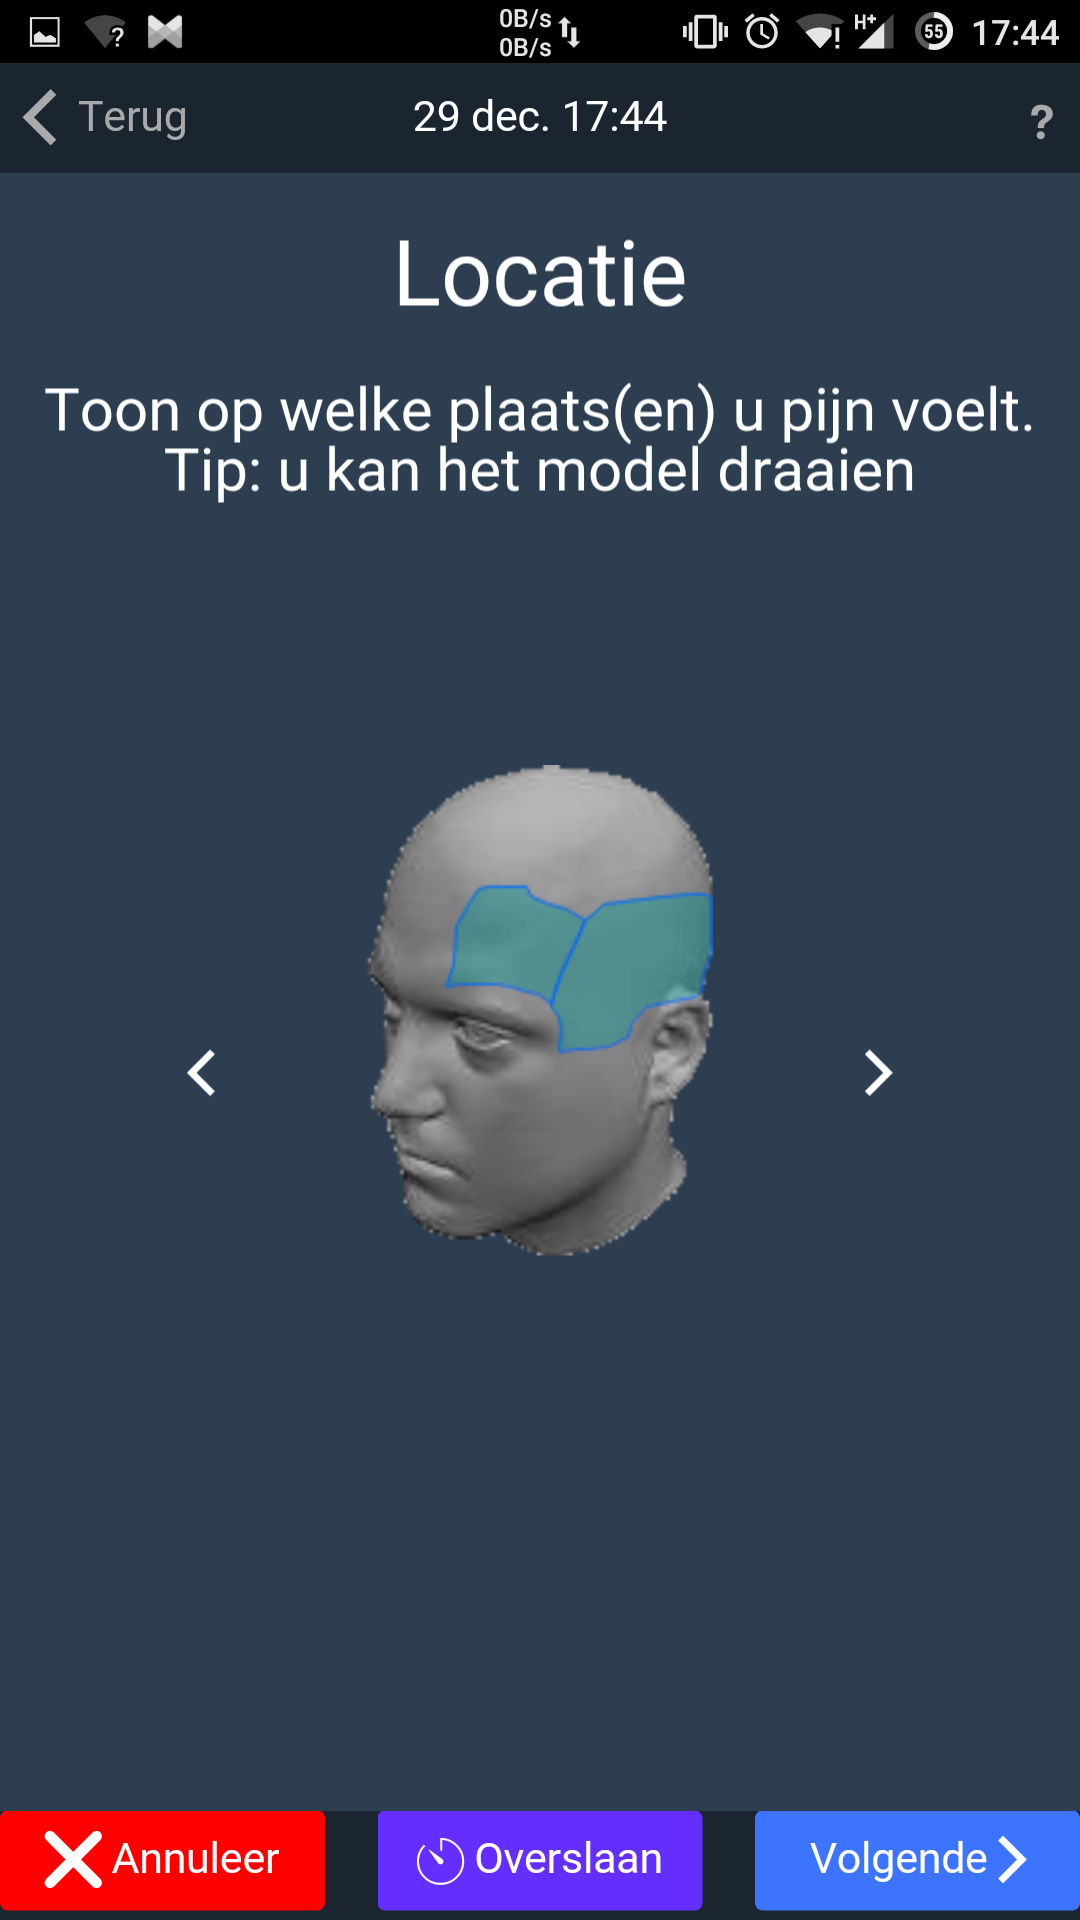
\includegraphics[width=\textwidth]{figures/add_headache_5.png}
	\end{subfigure}
	\pause
	~ %add desired spacing between images, e. g. ~, \quad, \qquad, \hfill etc. 
	%(or a blank line to force the subfigure onto a new line)
	\begin{subfigure}[b]{0.3\textwidth}
		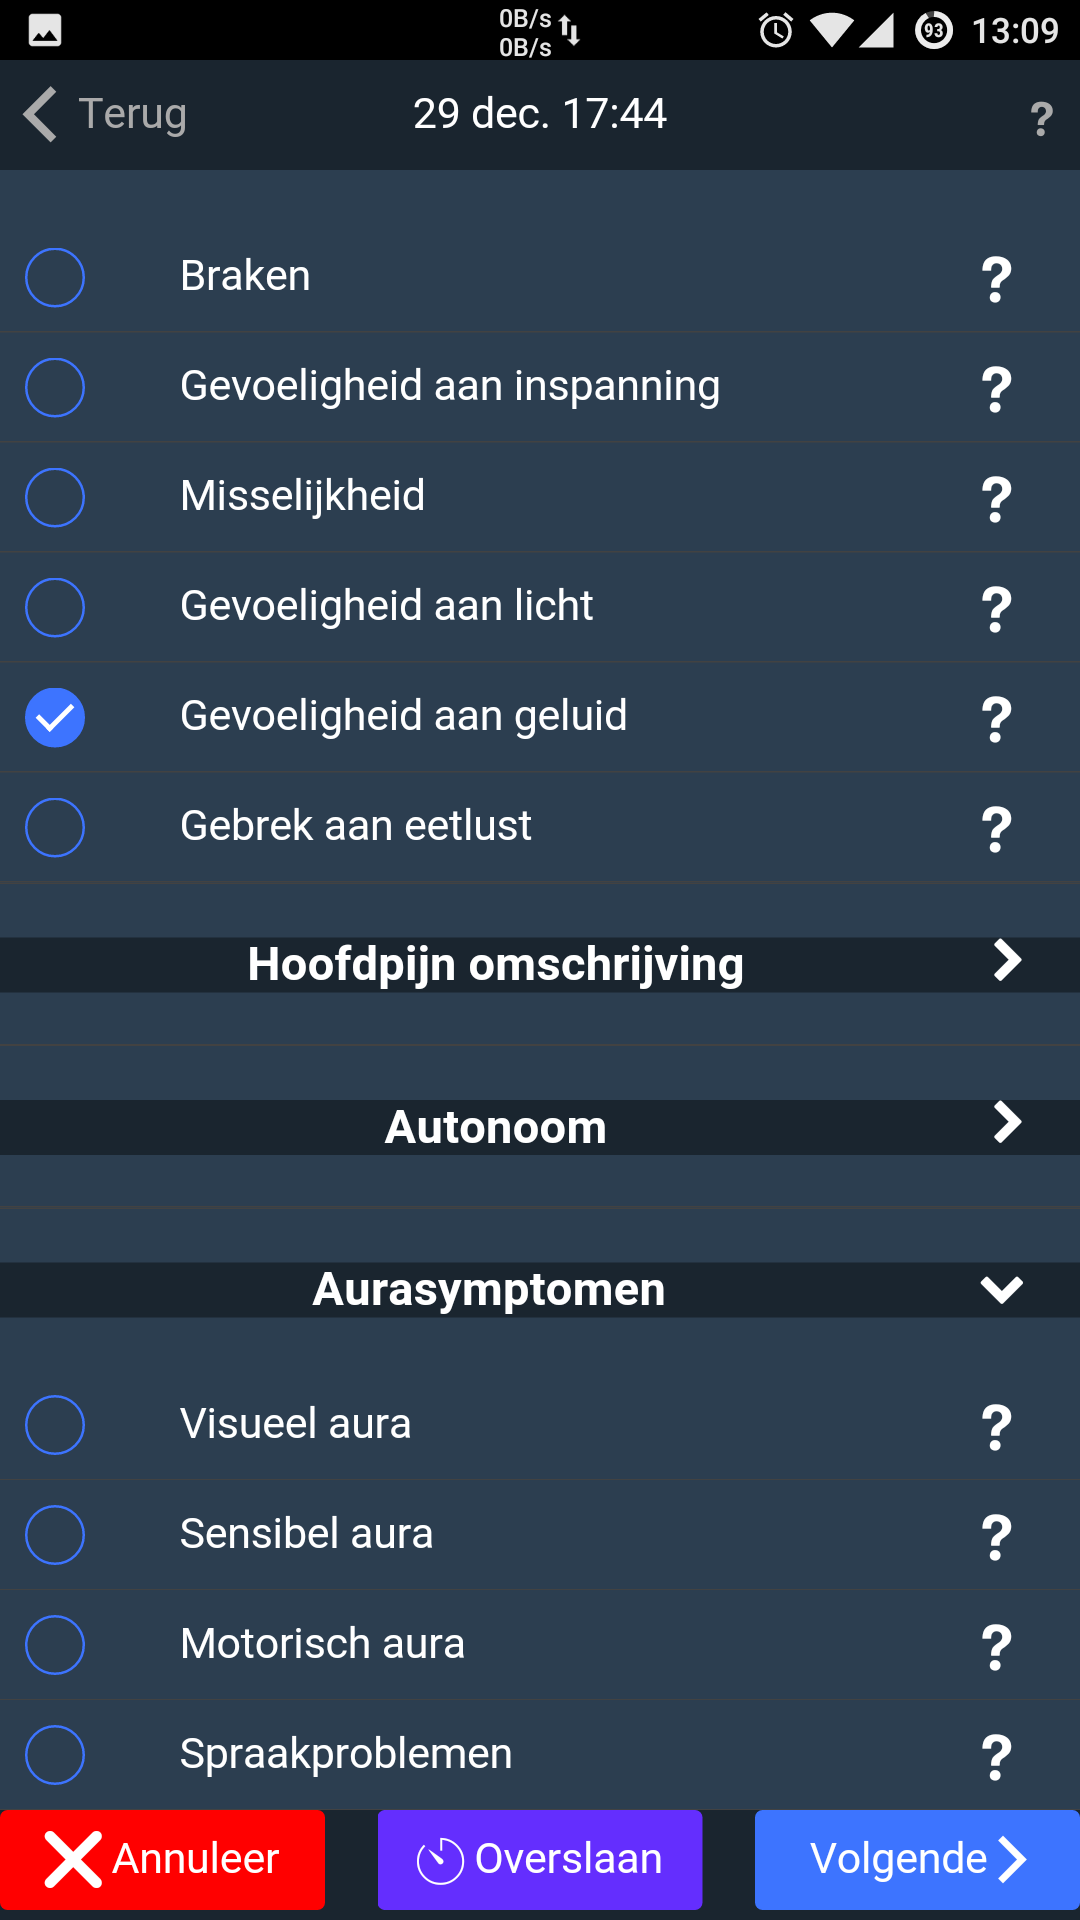
\includegraphics[width=\textwidth]{figures/add_headache_6.png}
	\end{subfigure}
	\pause
	~ %add desired spacing between images, e. g. ~, \quad, \qquad, \hfill etc. 
	%(or a blank line to force the subfigure onto a new line)
	\begin{subfigure}[b]{0.3\textwidth}
		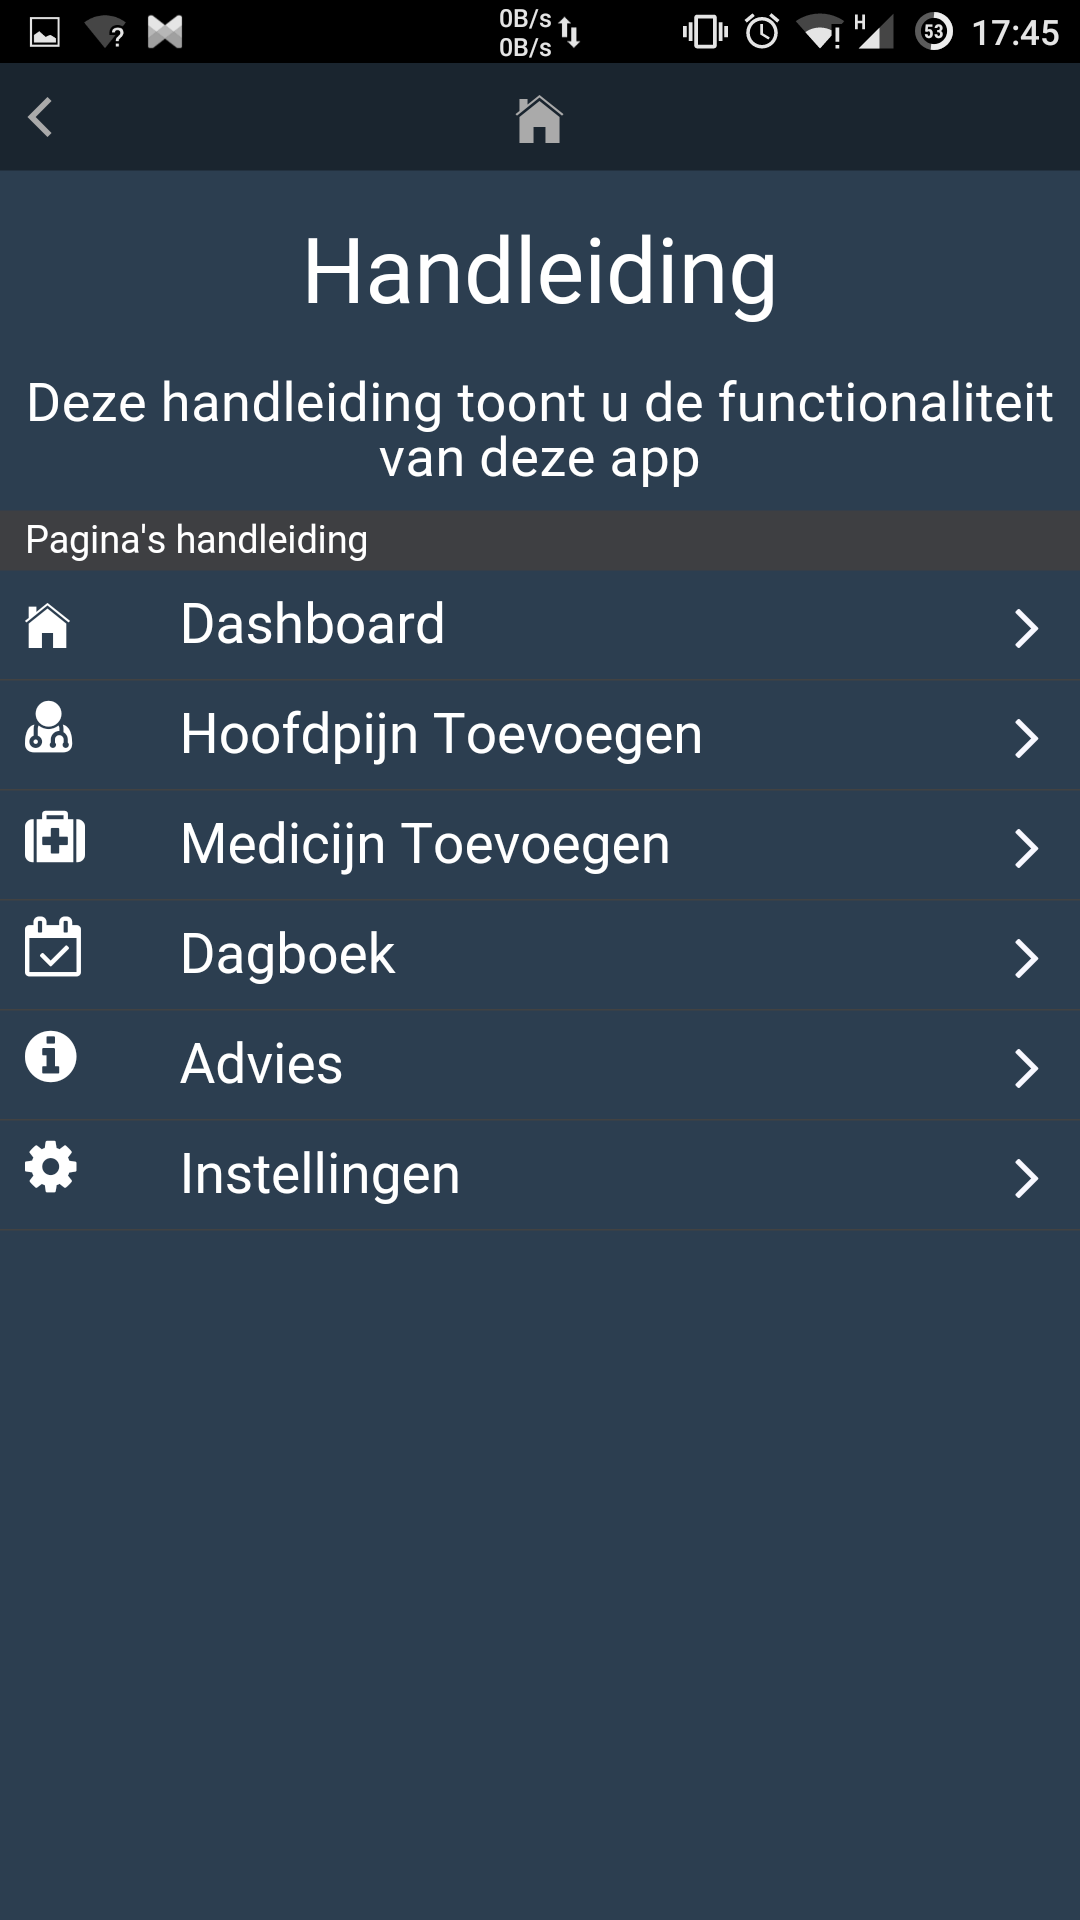
\includegraphics[width=\textwidth]{figures/manual.png}
	\end{subfigure}
\end{figure}
\end{frame}
\section{Backend and data exposure}
\begin{frame}{Backend and data exposure}
	\centering
	\begin{figure}
		\only<1>{		\includegraphics[width=\textwidth]{figures/system_analysis.png}}
		\only<2>{
			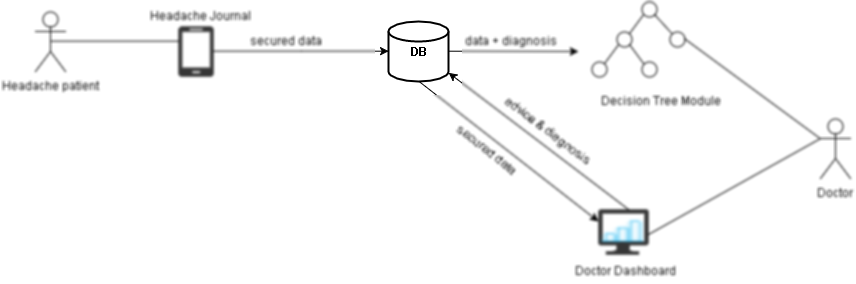
\includegraphics[width=\textwidth]{figures/system_analysis_backend.png}
		}
	\end{figure}
\end{frame}
\begin{frame}{Backend and data exposure}
	\begin{block}{Components}
		\begin{itemize}
			\item Database
			\item Connection to App
			\item Connection to Docter Dashboard
			\item Connection Machine learning module
		\end{itemize}
	\end{block}
\end{frame}
\begin{frame}{System}
	
	  \begin{center}
	  	\begin{tikzpicture}
	  	\node<1->[anchor=south west,inner sep=0] (image) at (0,0) {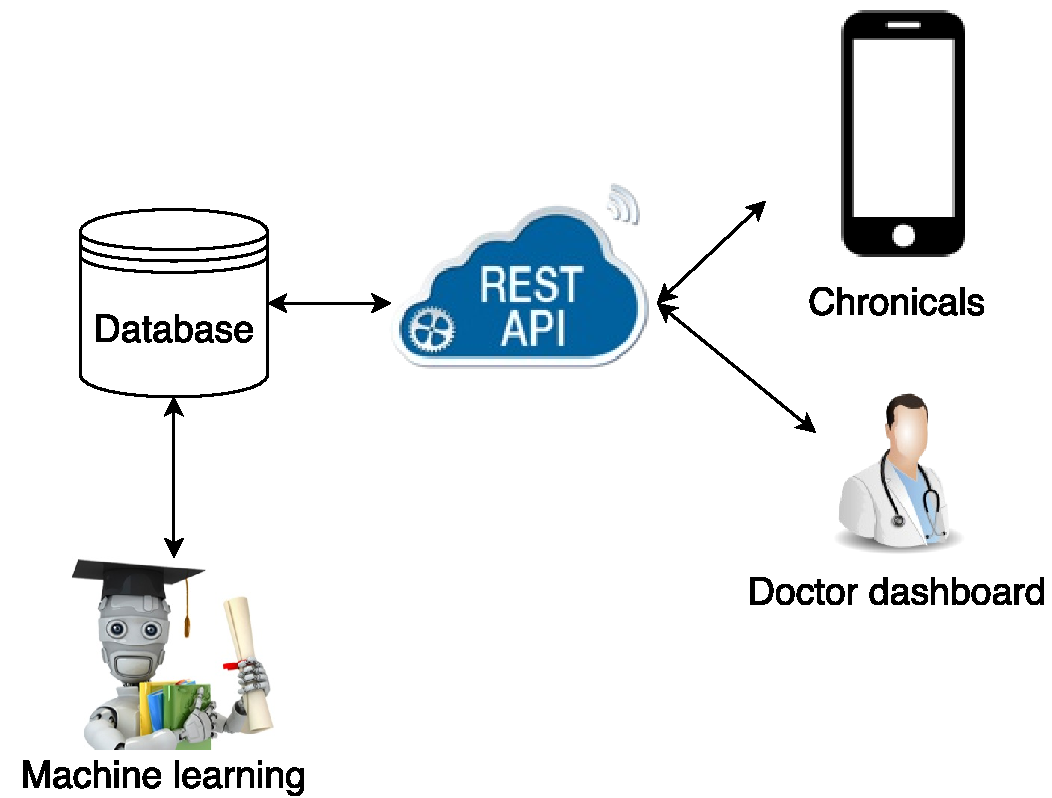
\includegraphics[width=0.6\textwidth]{figures/Data_exposure.pdf}};
	  	\node<2>[anchor=south west,inner sep=0] at (0,3.9) {
\includegraphics[width=0.2\textwidth]{figures/mongoDB.png}};
	  	\node<2>[anchor=south west,inner sep=0,red,font={\large\bfseries}] at (2.0,2.2) {Jax-RS(Java)};
	  	\end{tikzpicture}
	  \end{center}	
\end{frame}

\section{Machine learning}
\begin{frame}{Machine learning}
	\centering
	\begin{figure}
		\only<1>{		\includegraphics[width=\textwidth]{figures/system_analysis.png}}
		\only<2>{
			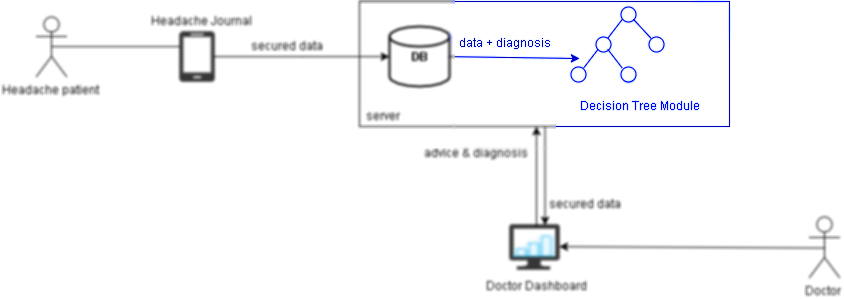
\includegraphics[width=\textwidth]{figures/system_analysis_ml.png}
		}
	\end{figure}
\end{frame}
\subsection*{Introduction}
\begin{frame}{Machine Learning}
	\only<2>{}
	Decision support ($\neq$ decision making) $\Rightarrow$ White box model
	\begin{block}{Possible models}
		\begin{itemize}
			\item {\color<2>{green} Decision trees}
			\item Random Forests (Gray box)
			\item Bayesian networks
		\end{itemize}
	\end{block}
\end{frame}
\begin{frame}{Genetic merging of DT's}
	\begin{columns}
		\begin{column}{0.25\textwidth}
			\centering
			\begin{figure}
				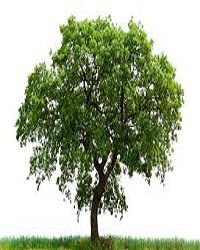
\includegraphics[width=\textwidth]{figures/oak.jpg}
				\caption{C4.5 (C5.0)}
			\end{figure}
		\end{column}
		\begin{column}{0.25\textwidth}
			\centering
			\begin{figure}
				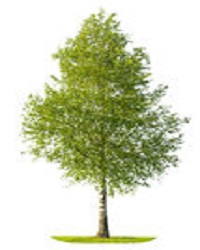
\includegraphics[width=\textwidth]{figures/berk.jpg}
				\caption{CART}
			\end{figure}
		\end{column}
		\begin{column}{0.25\textwidth}
			\centering
			\begin{figure}
				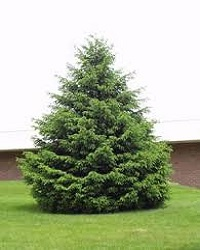
\includegraphics[width=\textwidth]{figures/spar.jpg}
				\caption{QUEST}
			\end{figure}
		\end{column}
		\begin{column}{0.25\textwidth}
			\centering
			$\ldots$
		\end{column}
	\end{columns}
	
	\textbf{$\rightarrow$ Which tree is the most beautiful?}
\end{frame}

\begin{frame}{Current ensembles lack interpretability}
	\begin{block}{}
	\textbf{Boosting, bagging, random forests,} etc. require majority voting (classification) or mean calculation (regression) to obtain prediction
	\end{block}
	
	\vspace{3em}
	\resizebox{0.24\textwidth}{!}{%
	\begin{tikzpicture}
	\node (A) [arn_l] {};
	\node (B) [arn_l, below left=0.75cm and 0.75 cm of A] {};
	\node (C) [arn_l, below right=0.75cm and 0.75 cm of A] {};
	\node (D) [rect_l, below left of=B] {0};
	\node (E) [rect_l, below right of=B] {1};
	\node (F) [rect_l, below left of=C] {1};
	\node (G) [rect_x, below right of=C] {0};
	\draw (A) -- (B);
	\draw (A) -- (C);
	\draw (B) -- (D);
	\draw (B) -- (E);
	\draw (C) -- (F);
	\draw (C) -- (G);
	\end{tikzpicture}%
	 } \resizebox{0.24\textwidth}{!}{%
		\begin{tikzpicture}
		\node (A) [arn_l] {};
		\node (B) [arn_l, below left=0.75cm and 0.75 cm of A] {};
		\node (C) [arn_l, below right=0.75cm and 0.75 cm of A] {};
		\node (D) [rect_l, below left of=B] {0};
		\node (E) [rect_l, below right of=B] {1};
		\node (F) [rect_l, below left of=C] {1};
		\node (G) [rect_x, below right of=C] {0};
		\draw (A) -- (B);
		\draw (A) -- (C);
		\draw (B) -- (D);
		\draw (B) -- (E);
		\draw (C) -- (F);
		\draw (C) -- (G);
		\end{tikzpicture}%
		 } \resizebox{0.24\textwidth}{!}{ %		
	 	$\ldots$ %
		}	\resizebox{0.24\textwidth}{!}{%
		\begin{tikzpicture}
		\node (A) [arn_l] {};
		\node (B) [arn_l, below left=0.75cm and 0.75 cm of A] {};
		\node (C) [arn_l, below right=0.75cm and 0.75 cm of A] {};
		\node (D) [rect_l, below left of=B] {0};
		\node (E) [rect_x, below right of=B] {1};
		\node (F) [rect_l, below left of=C] {1};
		\node (G) [rect_l, below right of=C] {0};
		\draw (A) -- (B);
		\draw (A) -- (C);
		\draw (B) -- (D);
		\draw (B) -- (E);
		\draw (C) -- (F);
		\draw (C) -- (G);
		\end{tikzpicture}%
		 }
	
	\framesubtitle{Stacking}
\end{frame}

\begin{frame}{Current ensembles lack interpretability}
	\begin{block}{}
		The final decision tree obtained by \textbf{stacking} contains uninterpretable internal nodes
	\end{block}
	
	\vspace{2em}
	
	\begin{tikzpicture}
	\centering
	\node (A) [rect_l] {$x_1 \leq 5.0$};
	\node (B) [rect_x, below left=0.75cm and 0.75 cm of A] {$outcome_{NN} \leq 2.0$};
	\node (C) [rect_x, below right=0.75cm and 0.75 cm of A] {$outcome_{RF} \leq 4.0$};
	\node (D) [rect_l, below left=0.5cm and 0.5cm of B] {0};
	\node (E) [rect_l, below right=0.5cm and 0.5cm of B] {1};
	\node (F) [rect_l, below left=0.5cm and 0.5cm of C] {0};
	\node (G) [rect_l, below right=0.5cm and 0.5cm of C] {1};
	\draw (A) -- (B);
	\draw (A) -- (C);
	\draw (B) -- (D);
	\draw (B) -- (E);
	\draw (C) -- (F);
	\draw (C) -- (G);
	\end{tikzpicture}
	
\end{frame}

\subsection*{Merging different DT's}

\begin{frame}{Decision tree $\rightarrow$ decision space}
	\begin{block}{Converting decision trees to decision spaces}
		We can define a one-to-one mapping between a decision tree and a set of $k$-dimensional hyperplanes ($k$ = $\#$features), called \textbf{decision~space}.	Each node in the decision tree corresponds to a hyperplane in the decision space.
	\end{block}
\end{frame}

\begin{frame}{Decision tree $\rightarrow$ decision space}
	\begin{figure}
		\centering
		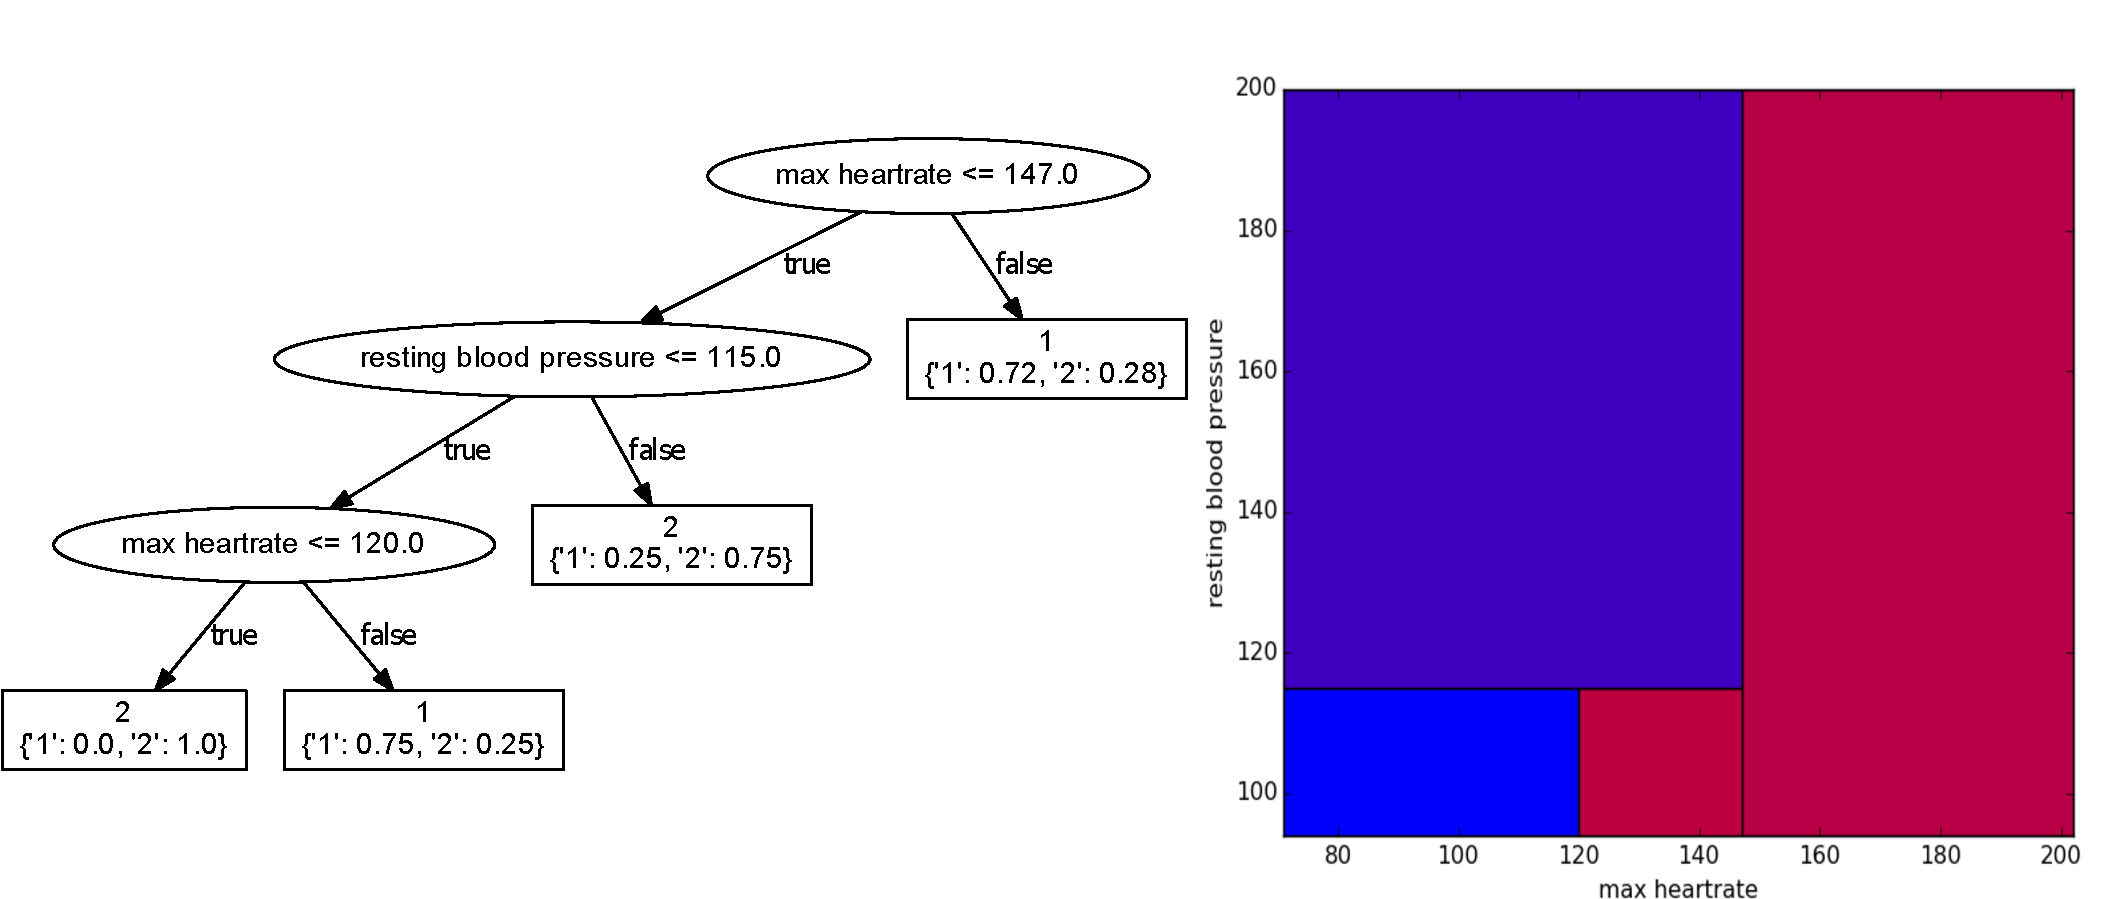
\includegraphics[width=\textwidth]{figures/dt_to_space.pdf}
	\end{figure}
\end{frame}

\begin{frame}{Merging decision spaces}
	\frametitle<1>{Merging decision spaces}
	\frametitle<3>{Pruning decision spaces}
	\only<1>{
		
		\begin{figure}
			\centering
			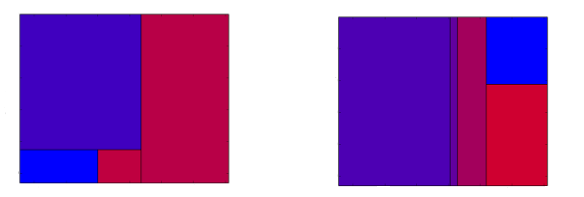
\includegraphics[width=\textwidth]{figures/merge_space_1.png}
		\end{figure}
	}
	\only<2>{

		\begin{figure}
			\centering
			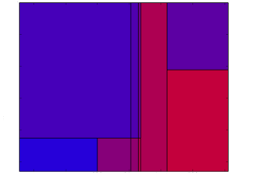
\includegraphics[scale=1]{figures/merge_space_2.png}
		\end{figure}
	}
	\onslide<3>{
		
		\begin{figure}
			\centering
			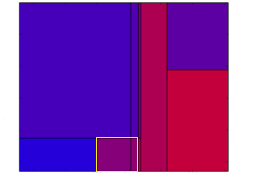
\includegraphics[scale=1]{figures/pruning.png}
		\end{figure}
	}
\end{frame}


\begin{frame}{Decision space $\rightarrow$ decision tree}
	\begin{block}{Converting decision spaces to decision trees}
		One-to-one mapping from decision tree to space is lost during conversion because the order is lost. Therefore, a \textbf{heuristic} approach must be taken, identifying \textbf{hyperplane candidates} and calculating a metric to choose the `best' plane.
	\end{block}
\end{frame}

\begin{frame}{Decision space $\rightarrow$ decision tree}
	\only<1>{
		\begin{figure}
			\centering
			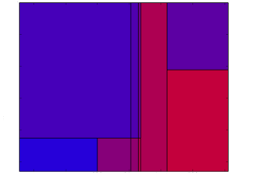
\includegraphics[scale=1]{figures/merge_space_2.png}
		\end{figure}	
	}
	\only<2>{
		\begin{figure}
			\centering
			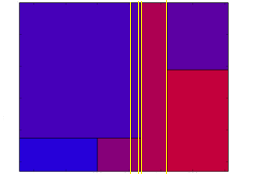
\includegraphics[scale=1]{figures/space_to_dt.png}
		\end{figure}	
	}
\end{frame}

\begin{frame}{Decision space $\rightarrow$ decision tree}
	\begin{block}{Finding `best' candidate hyperplane}
		Apply metric function to each plane, these include:
		\begin{itemize}
			\item information gain and Gini
			\item pick plane from most correlated feature
			\item pick plane that divide space in two most equal subspaces
			\item combination
		\end{itemize}
	\end{block}
	
\end{frame}


\subsection*{Genetic algorithm}
{\setbeamertemplate{footline}{}
\begin{frame}{}
	\begin{figure}
		\centering
		\includegraphics[scale=0.33]{figures/genetic.png}
	\end{figure}	
\end{frame} }

\begin{frame}{Splitting the data}
	\vspace{-1em}
	\begin{figure}
		\centering
		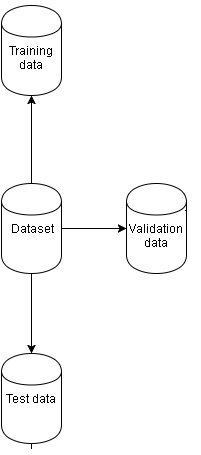
\includegraphics[scale=0.5]{figures/split_data.png}
	\end{figure}	
\end{frame}

\begin{frame}{Generate different decision trees}
	\begin{figure}
		\centering
		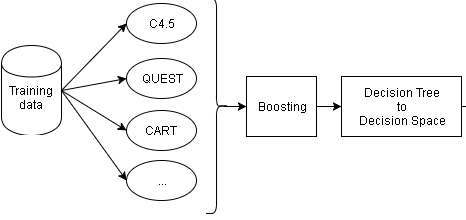
\includegraphics[scale=0.8]{figures/generate_dt.png}
	\end{figure}	
\end{frame}

\begin{frame}{Generate different decision trees}
	\begin{figure}
		\centering
		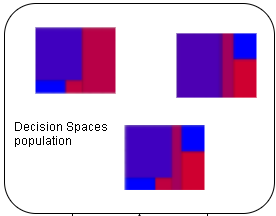
\includegraphics[scale=1]{figures/dt_population.png}
	\end{figure}	
\end{frame}

{\setbeamertemplate{footline}{}
\begin{frame}{Genetic merging}
	\begin{figure}
		\centering
		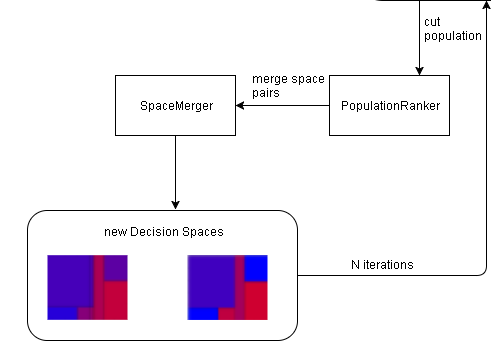
\includegraphics[scale=0.7]{figures/genetic_merging.png}
	\end{figure}
\end{frame} }

\begin{frame}{PopulationRanker}
	\begin{block}{Fitness function}
		A high accuracy is the most important property of a decision tree, followed by its' size ($\rightarrow$ comprehensibility). Genetic algorithms are well suited for \textbf{multi-objective optimization}.
	\end{block}
\end{frame}

{\setbeamertemplate{footline}{}
\begin{frame}{Final iteration}
	\vspace{-1em}
	\begin{figure}
		\centering
		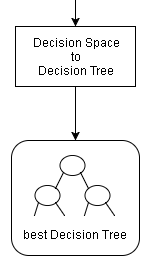
\includegraphics[scale=1]{figures/final_iteration.png}
	\end{figure}
\end{frame} }

\begin{frame}{Headache dataset}
	Data collection could only start in March: \\
	\begin{itemize}
		\item the mobile application had to be finished first
		\item an ethical committee had to approve our application
	\end{itemize} \vspace{2em}
	$\rightarrow$ too few samples for machine learning
\end{frame}

\begin{frame}
	\begin{figure}
		\centering
			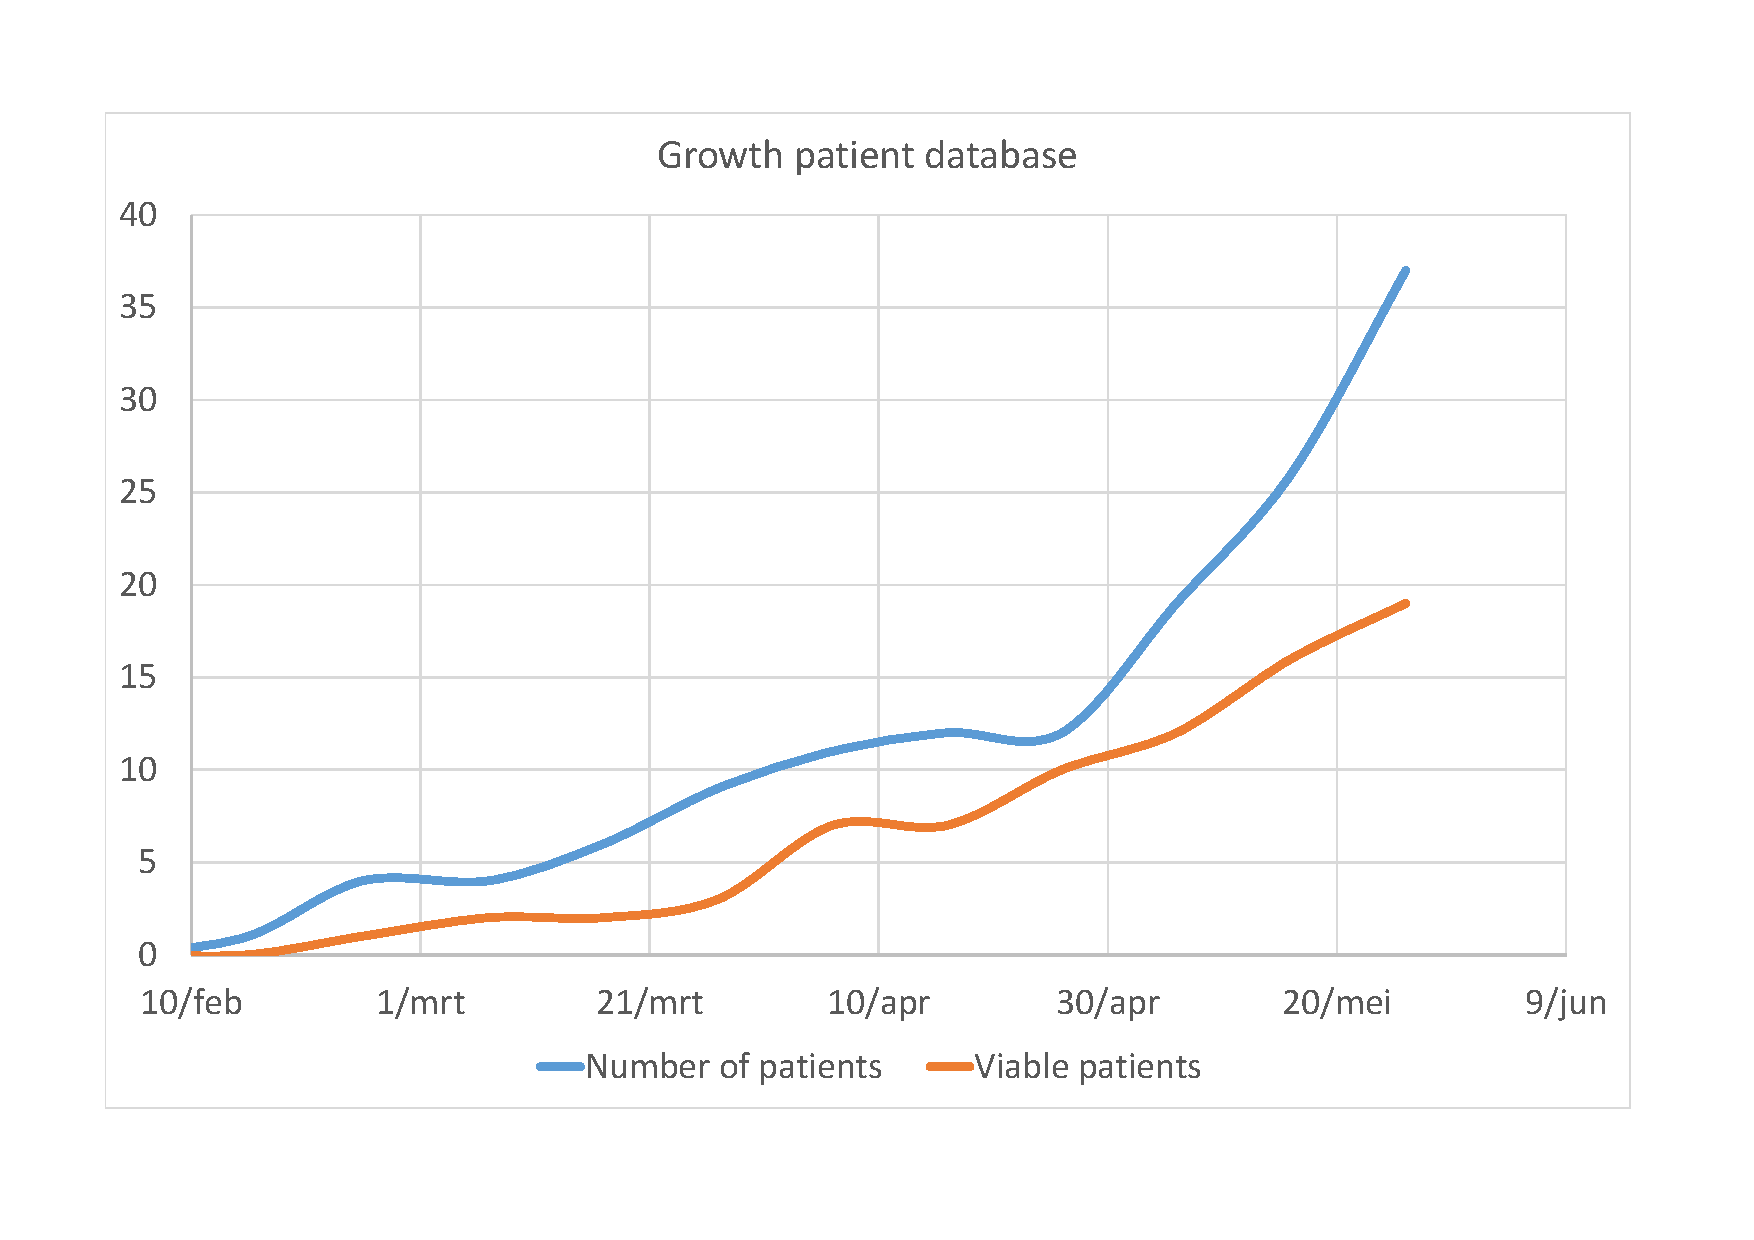
\includegraphics[width=\textwidth]{figures/chart_patients.pdf}
	\end{figure}

\end{frame}

\begin{frame}{Evaluating our algorithm}
	\begin{block}{}
		5 datasets from UCI \\
		optimal parameters, feature selection when needed and k-fold CV
	\end{block}
\begin{adjustwidth}{-0.4cm}{}
	\begin{table}
			\begin{tabular}{l|ccccc}
				\textbf{Name}    & \multicolumn{1}{l}{\textbf{\#Samples}} & \multicolumn{1}{l}{\textbf{\#Disc}} & \multicolumn{1}{l}{\textbf{\#Cont}} & \multicolumn{1}{l}{\textbf{\#Class}} & \multicolumn{1}{l}{\textbf{Imbalance rate}} \\ \hline
				\textbf{Heart}   & 270                                    & 7                                   & 6                                   & 2                                      & 0.058                                       \\
				\textbf{Car}     & 1728                                   & 6                                   & 0                                   & 4                                      & 0.225                                       \\
				\textbf{Iris}    & 150                                    & 0                                   & 4                                   & 3                                      & 0                                           \\
				\textbf{Shuttle} & 14500                                  & 0                                   & 9                                   & 7                                      & 0.18308                                     \\
				\textbf{Nursery} & 12960                                  & 8                                   & 0                                   & 5                                      & 0.1498      
			\end{tabular}
		\end{table}
	\end{adjustwidth}
\end{frame}
%
%\begin{frame}{Heart disease dataset}
%	\begin{columns}
%		\begin{column}{0.35\textwidth}
%			\begin{figure}
%				\centering
%				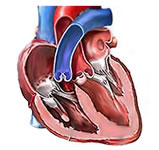
\includegraphics[scale=0.75]{figures/heart.jpg}
%			\end{figure}
%		\end{column}
%		
%		\begin{column}{0.65\textwidth}
%			\begin{itemize}
%				\item medical dataset
%				\item 270 samples
%				\item 13 features: 6 continuous (max heartrate), 7 discrete (sex)
%				\item 2 classes: sick or healthy
%				\item more healthy than sick samples
%				\item false negatives can cost lives!
%			\end{itemize}
%		\end{column}
%	\end{columns}
%\end{frame}
%
%\begin{frame}{Car evaluation dataset}
%	\begin{columns}
%		\begin{column}{0.35\textwidth}
%			\begin{figure}
%				\centering
%				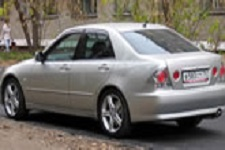
\includegraphics[scale=1]{figures/car.jpg}
%			\end{figure}
%		\end{column}
%		
%		\begin{column}{0.65\textwidth}
%			\begin{itemize}
%				\item 1725 samples
%				\item only 6 features, all categories (price, doors, $\ldots$)
%				\item 4 classes: unacceptable, acceptable, good and very good
%				\item VERY imbalanced (70\% unacc, 22.2\% acc)
%			\end{itemize}
%		\end{column}
%	\end{columns}
%\end{frame}
%
%\begin{frame}{Iris flowers dataset}
%	\begin{columns}
%		\begin{column}{0.35\textwidth}
%			\begin{figure}
%				\centering
%				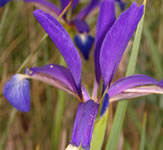
\includegraphics[scale=0.75]{figures/iris.jpg}
%			\end{figure}
%		\end{column}
%		
%		\begin{column}{0.65\textwidth}
%			\begin{itemize}
%				\item very small dimensions
%				\item 150 flowers
%				\item 4 continuous features (petal width and sepal length)
%				\item 3 classes: setosa, versicolor, virginica
%				\item perfectly balanced (50-50-50)
%			\end{itemize}
%		\end{column}
%	\end{columns}
%\end{frame}
%
%\begin{frame}{Shuttle classification dataset}
%	\begin{columns}
%		\begin{column}{0.35\textwidth}
%			\begin{figure}
%				\centering
%				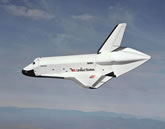
\includegraphics[scale=0.75]{figures/shuttle.jpg}
%			\end{figure}
%		\end{column}
%		
%		\begin{column}{0.65\textwidth}
%			\begin{itemize}
%				\item originally: 58000 samples corresponding to aircrafts
%				\item here: 14500 samples
%				\item 9 numerical attributes
%				\item 7 different types of shuttles: 2 of them contained less than 10 samples (discarded)
%			\end{itemize}
%		\end{column}
%	\end{columns}
%\end{frame}
%
%\begin{frame}{Nursery application dataset}
%	\begin{columns}
%		\begin{column}{0.35\textwidth}
%			\begin{figure}
%				\centering
%				
\includegraphics[scale=0.75]{figures/nursery.jpg}
%			\end{figure}
%		\end{column}
%		
%		\begin{column}{0.65\textwidth}
%			\begin{itemize}
%				\item 12960 samples (applications for nursery school)
%				\item 8 categorical features
%				\item 5 classes: not recommended, recommended, very recommended, priority and special priority
%				\item only 2 samples were recommended (discarded)
%			\end{itemize}
%		\end{column}
%	\end{columns}
%\end{frame}

{\setbeamertemplate{footline}{\leavevmode%
		\hbox{%
			\begin{beamercolorbox}[wd=.333333\paperwidth,ht=2.25ex,dp=1ex,center]{author in head/foot}%
				\usebeamerfont{author in head/foot}\insertsection
			\end{beamercolorbox}%
			\begin{beamercolorbox}[wd=.333333\paperwidth,ht=2.25ex,dp=1ex,center]{title in head/foot}%
				\usebeamerfont{title in head/foot}\insertsubsection
			\end{beamercolorbox}%
			\begin{beamercolorbox}[wd=.333333\paperwidth,ht=2.25ex,dp=1ex,right]{date in head/foot}%
				%			\usebeamerfont{date in head/foot}\insertshortdate{}\hspace*{2em}
				\insertframenumber{} / \inserttotalframenumber\hspace*{2ex} 
			\end{beamercolorbox}}%
			\vskip0pt%
		}
	\begin{frame}{}
		\vspace{-0.75em}
		\only<1>{
			\begin{table}
				\begin{tabular}{|c|c|c|c|c|c|}
					\hline \textbf{Dataset} & \textbf{Folds} & \textbf{C4.5} & \textbf{CART} & \textbf{QUEST} & \textbf{Genetic} \\ \hline
					\multirow{2}{*}{Heart disease} & 5 & \underline{$\textbf{0.8067}$} & $0.7844$ & $0.7844$ & \underline{$\textbf{0.8067}$} \\
					& 10 & \underline{$\textbf{0.8104}$} & $0.7732$ & $0.7881$ & $0.7993$ \\ \hline
					\multirow{2}{*}{Iris} & 3 & $0.9533$ & $0.9467$ & $0.9467$ & \underline{$\textbf{0.96}$} \\ & 5 & $0.9467$ & $0.9333$ & $0.9467$ & \underline{$\textbf{0.9533}$} \\ \hline
					\multirow{3}{*}{Cars} & 3 & \underline{$\textbf{0.9722}$} & $0.9693$ & $0.9229$ & $0.9693$ \\
					& 5 & $0.9711$ & $0.9682$ & $0.9241$ & \underline{$\textbf{0.9786}$} \\
					& 10 & $0.9756$ & $0.9751$ & $0.9265$ & \underline{$\textbf{0.9803}$} \\ \hline
					\multirow{3}{*}{Shuttle} & 3 & $0.9987$ & $0.9983$ & $0.9964$ & \underline{$\textbf{0.9988}$}  \\
					& 5 & $0.9986$ & $0.9981$ & $0.9962$ & \underline{$\textbf{0.9988}$} \\
					& 10 & $0.9990$ & $0.9987$ & $0.9941 $ & \underline{$\textbf{0.9992}$} \\ \hline
					\multirow{3}{*}{Nursery} & 3 & $0.9890$ & $0.9431$ & $0.9147$ & \underline{$\textbf{0.9914}$} \\
					& $5$ & $0.9918$ & $0.9498$ & $0.9251$ & \underline{$\textbf{0.9958}$} \\
					& 10 & $0.9937$ & $0.9568$ & $0.9259$ & \underline{$\textbf{0.9954}$} \\ \hline
				\end{tabular}
			\end{table}	
		}
		\only<2>{
			\begin{figure}
				\centering
				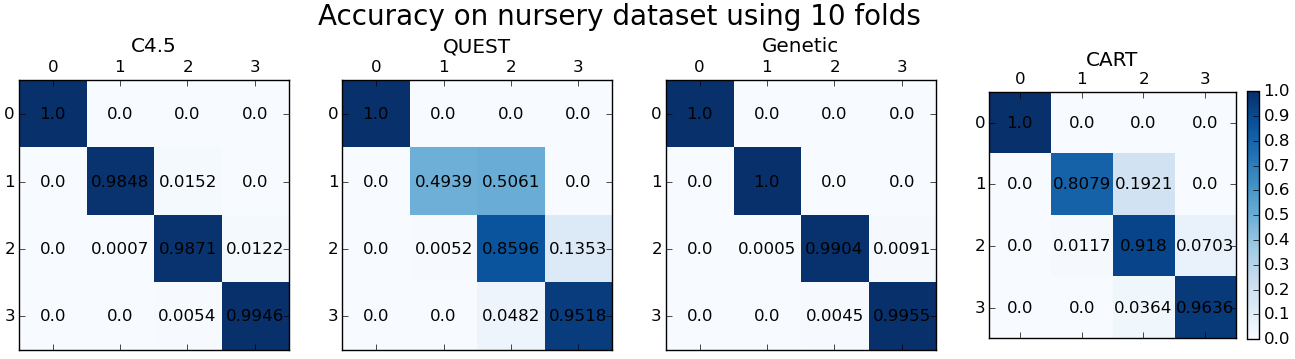
\includegraphics[scale=0.42]{figures/genetic_nurse_10_folds.png}
			\end{figure}
		}
	\end{frame} }

\section{Doctor dashboard}
\begin{frame}{Doctor dashboard}
	\centering
	\begin{figure}
		\only<1>{		\includegraphics[width=\textwidth]{figures/system_analysis.png}}
		\only<2>{
			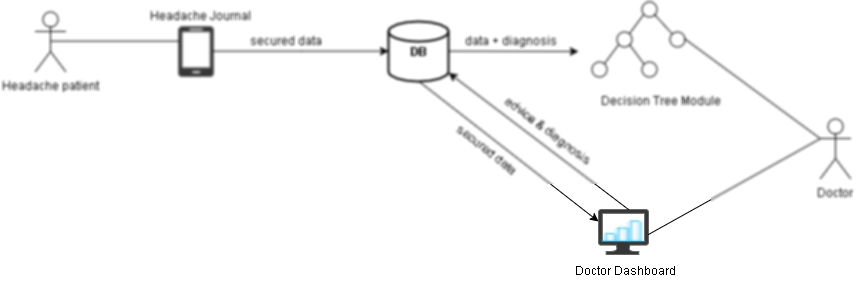
\includegraphics[width=\textwidth]{figures/system_analysis_doctor_dashboard.png}
		}
	\end{figure}
\end{frame}
\begin{frame}{Doctor Dashboard}
	\begin{itemize}
		\item Web application in order for the doctors to access the data exposed by our REST API \\
		\item Preferably in the form of visualizations, which allow to process a lot of data in a small amount of time
		\item Developed by Maarten Vanden Berghe
	\end{itemize}
%	\textbf{\Large Maarten Vanden Berghe}
%	\only<1>{
%		\begin{figure}
%			\centering
%			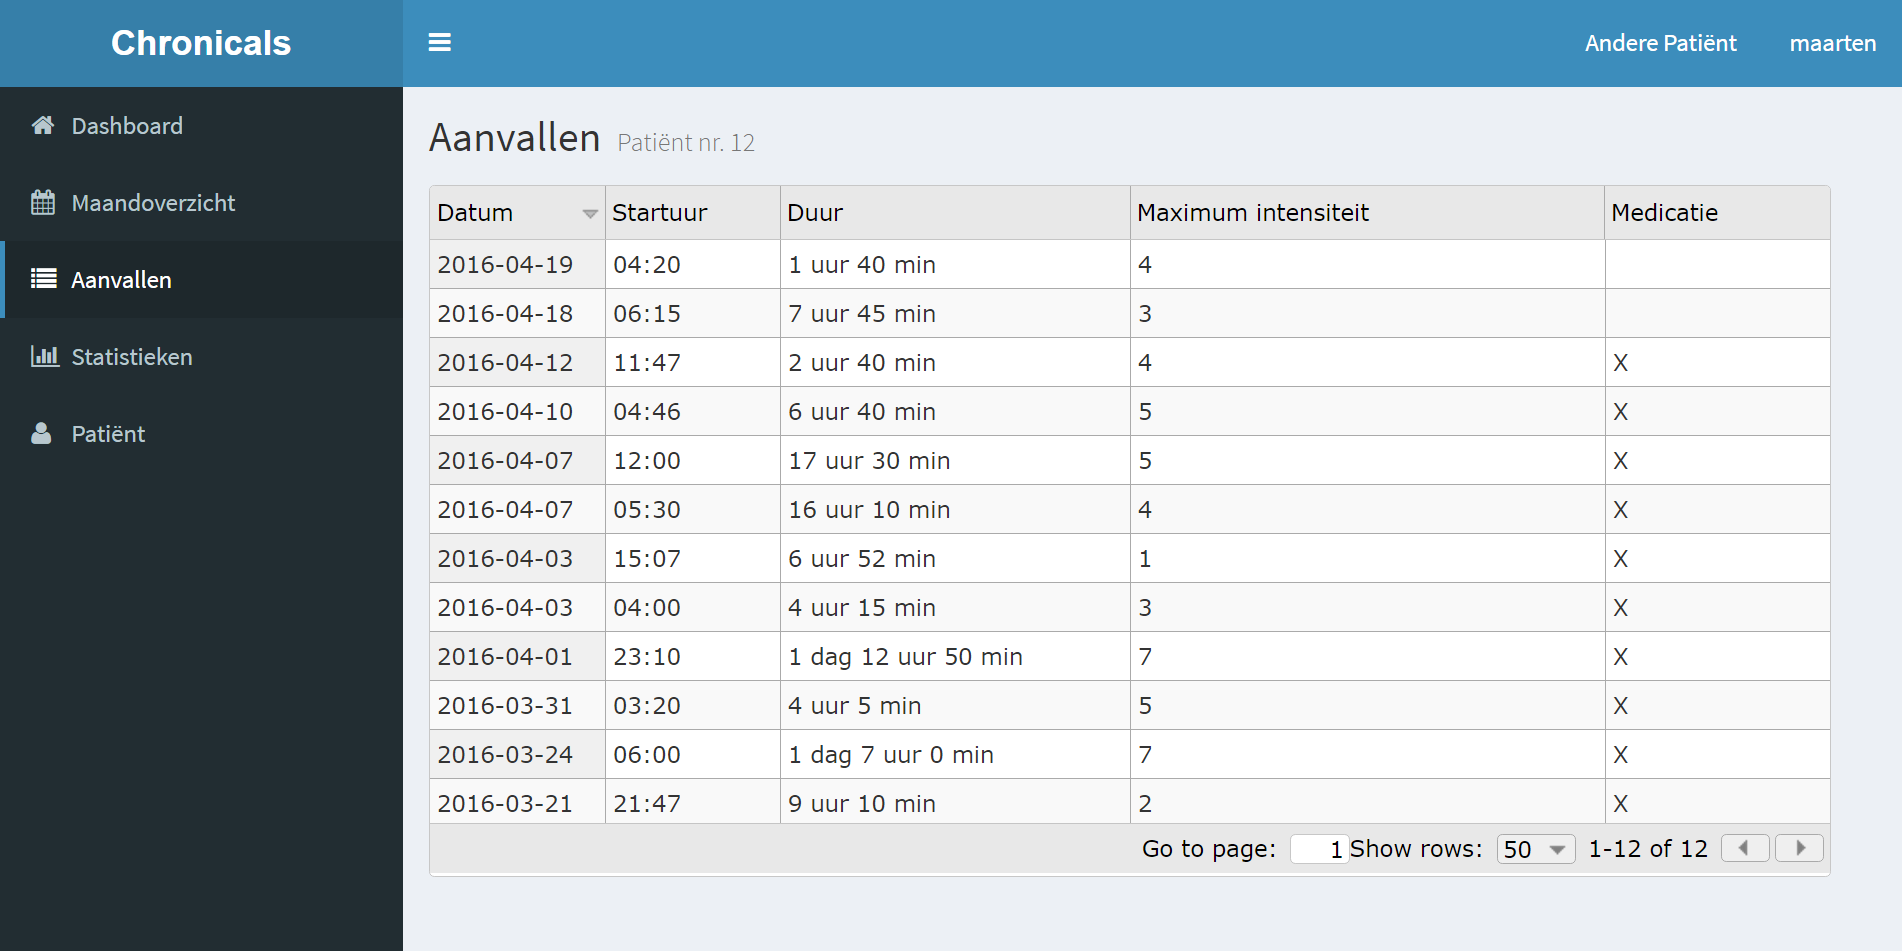
\includegraphics[width=\textwidth]{figures/aanvallen.png}
%		\end{figure}
%	}
%	
%	\only<2>{
%		\begin{figure}
%			\centering
%			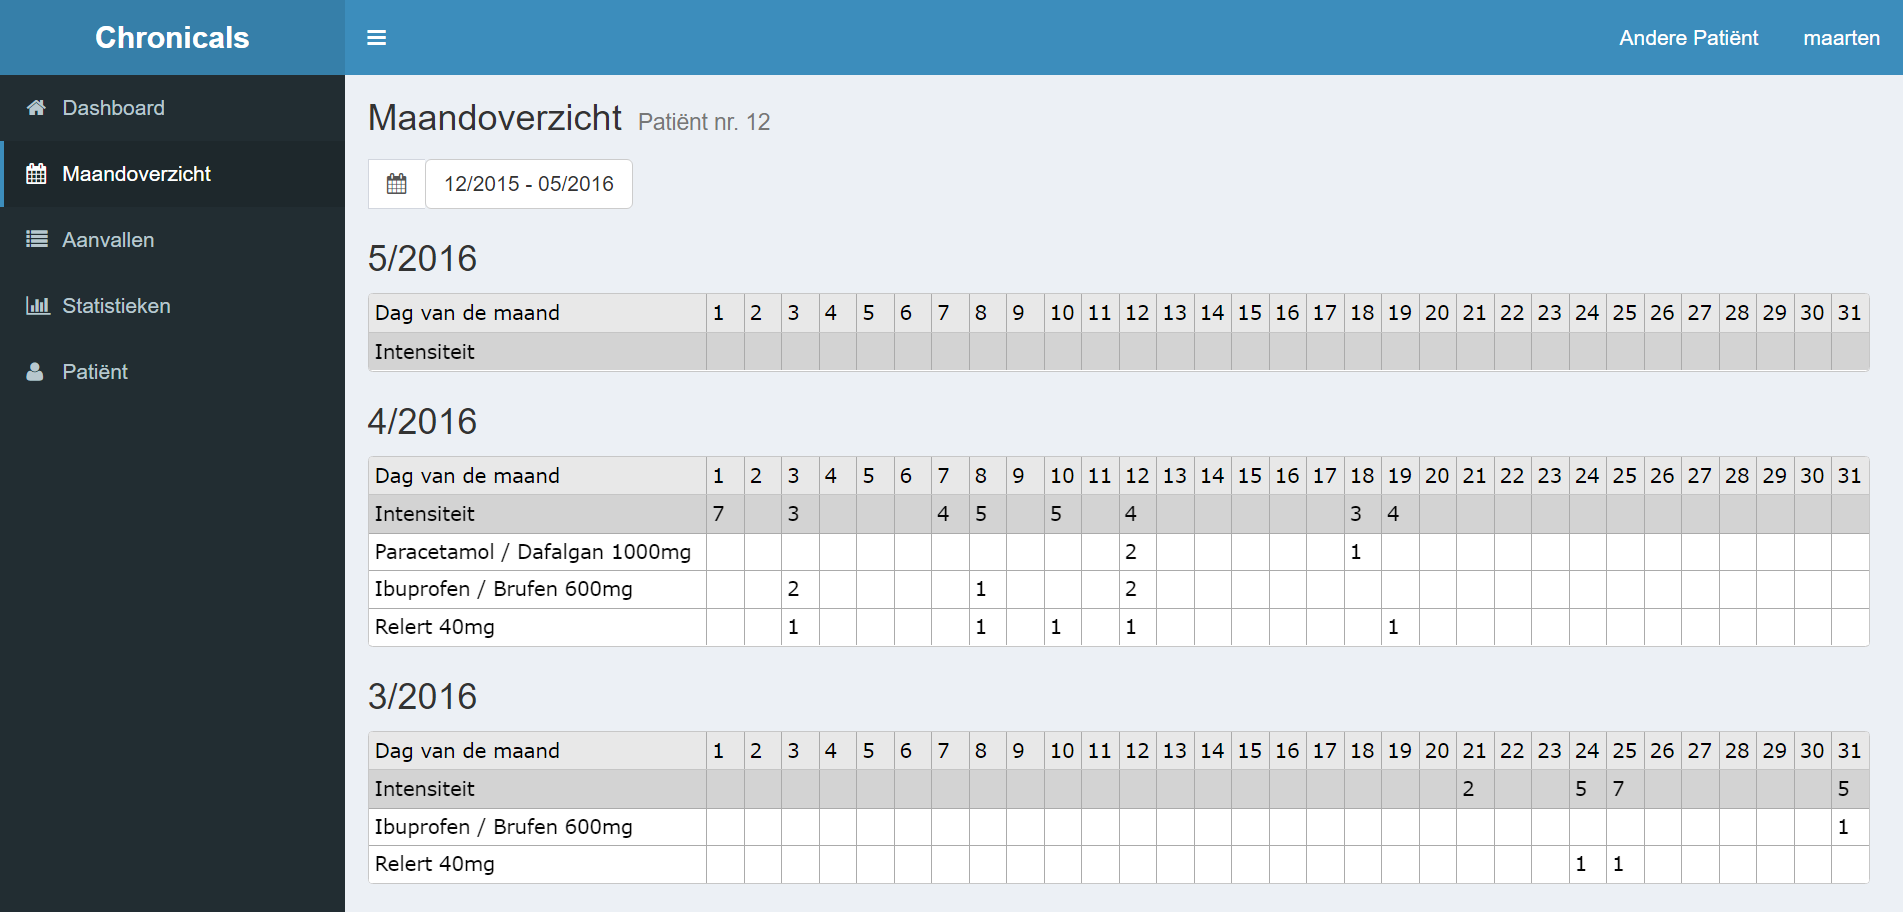
\includegraphics[width=\textwidth]{figures/maandoverzicht.png}
%		\end{figure}
%	}
%	
%	\only<3>{
%		\begin{figure}
%			\centering
%			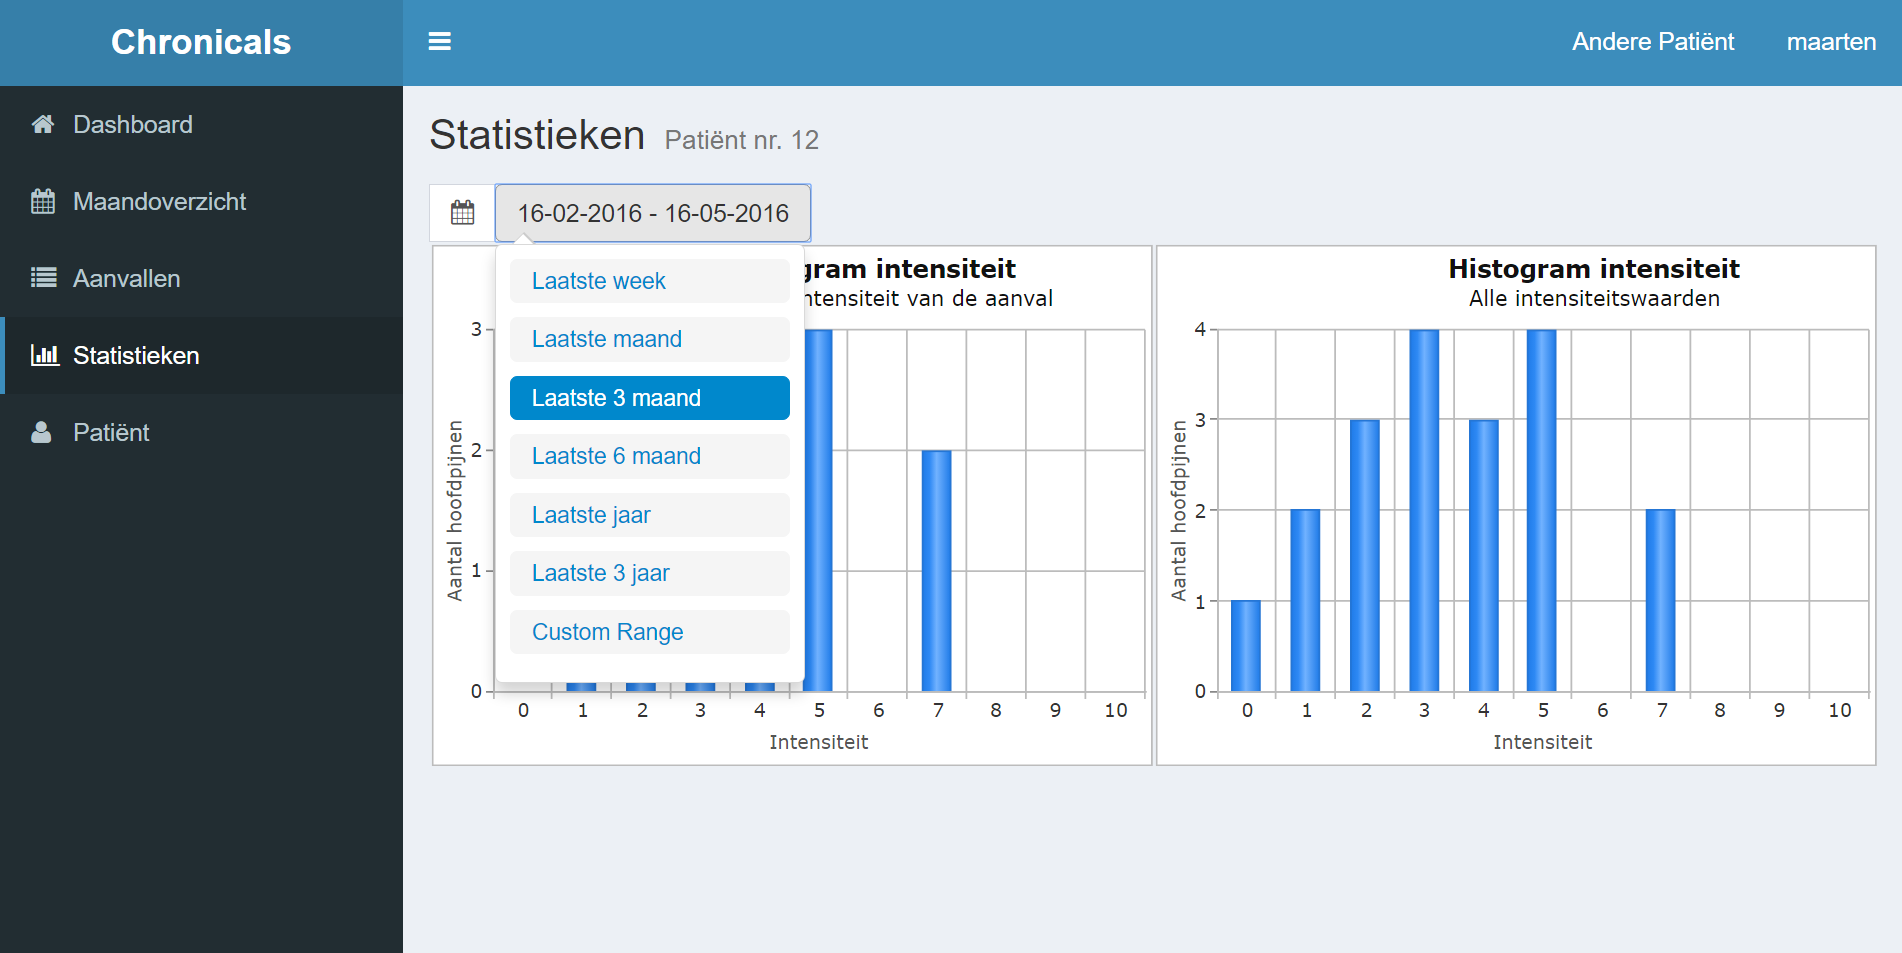
\includegraphics[width=\textwidth]{figures/statistieken2.png}
%		\end{figure}
%	}
%	
%	\only<4>{
%		\begin{figure}
%			\centering
%			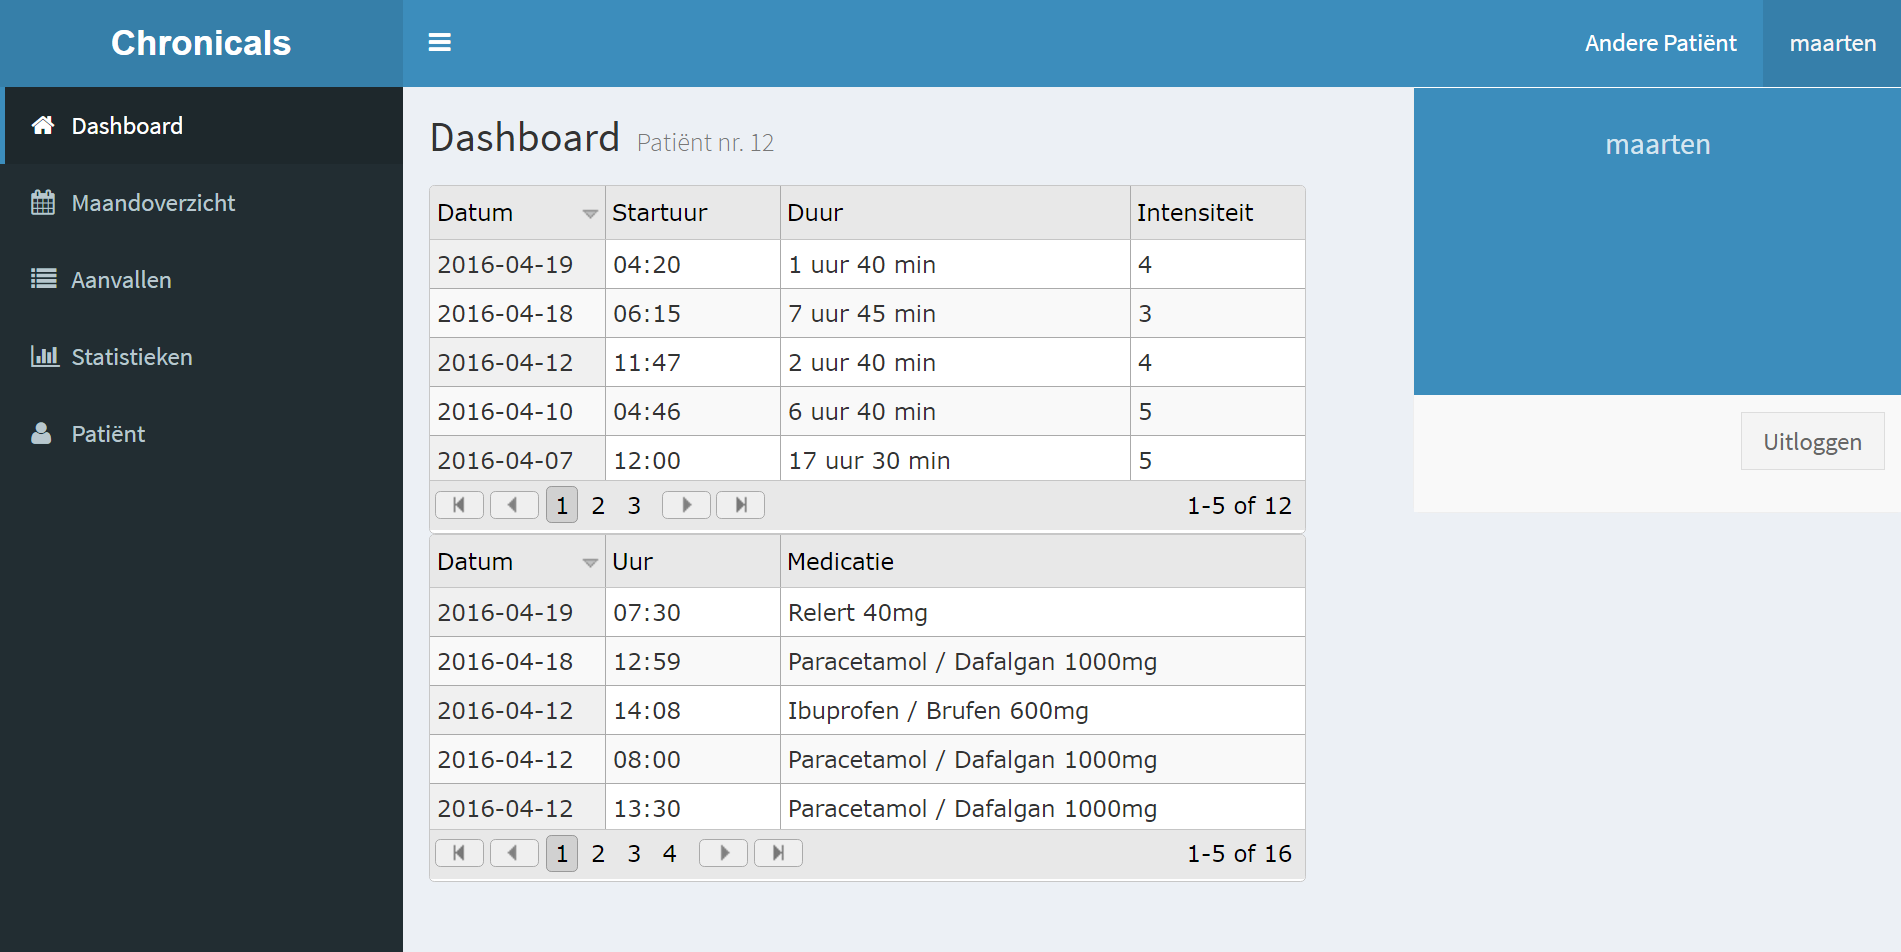
\includegraphics[width=\textwidth]{figures/uitloggen.png}
%		\end{figure}
%	}
\end{frame}
\section{Conclusion \& future work}




% subsection rstar (end)

% section concensusTeees (end)


\begin{frame}{Conclusion}
	\begin{itemize}
		\item It is shown that the current procces in the UH of Ghent can be completely digitized. Our solution can significantly improve the efficiency and reduce the frequency of consults, leading to a reduction
		in health care costs. \vspace{2em}
		\item The foundations for a diagnosis support system are built, using a genetic approach to merge different induced decision trees to obtain a single decision tree with enhanced accuracy.
	\end{itemize}
\end{frame}

\begin{frame}{Future work}
	\begin{itemize}
		\item Develop native applications for iOS and Android to enhance look-\&-feel
		\item Re-evaluate our machine learning models on a larger headache dataset
		\item Implement more induction algorithms and ensemble techniques to create a more diverse initial population
		\item Experiment with other selection techniques
		and fitness functions
		\item Optimize the heuristic approach to convert decision spaces to decision trees
	\end{itemize}
\end{frame}

{\setbeamertemplate{footline}{}
\begin{frame}{Thank you for your attention!}
	\scriptsize{\tableofcontents[hidesubsections]}
\end{frame} }


\end{document}